%-------------------------------------------------------------------------------
% Preamble
%-------------------------------------------------------------------------------

\documentclass{article}


%Packages
\usepackage{
	siunitx, % units
  graphicx, % for images
	natbib,
	booktabs
}
\usepackage[letterpaper]{geometry}
\renewcommand{\thefigure}{S\arabic{figure}}
\renewcommand{\thetable}{S\arabic{table}}
\usepackage[breaklinks=true,hidelinks]{hyperref}
\graphicspath{{../figs/}}

%-------------------------------------------------------------------------------
% Title and Authors
%-------------------------------------------------------------------------------

\title{Supplemental Information for\\``Heavy rainfall in Paraguay during the 2015-2016 austral summer: causes and subseasonal-to-seasonal predictive skill''}
\author{James Doss-Gollin\and \'{A}ngel G. Mu\~{n}oz  \and Simon J. Mason \and Max Past\'{e}n }
\date{\today}

\begin{document}

%% Necessary!
\maketitle

This document contains several supplemental figures described in the main text.
Further supporting information is available in the form of source code and \texttt{jupyter} notebooks at \url{github.com/jdossgollin/PYFloods}.

\listoftables
\listoffigures

\clearpage

\begin{table}
	\centering
	\begin{tabular}{lrr}
	\toprule
	{} &  NDJF 2015-16 &  Climatology \\
	WT &           &              \\
	\midrule
	1     &  0.258 &     0.212 \\
	2     &  0.242 &     0.187 \\
	3     &  0.133 &     0.158 \\
	4     &  0.192 &     0.155 \\
	5     &  0.092 &     0.146 \\
	6     &  0.083 &     0.142 \\
	\bottomrule
	\end{tabular}
	\caption{Weather type (WT) occurrence fraction during NDJF 2015-16 and Climatology}
\end{table}

\clearpage

\begin{figure}
	\centering
  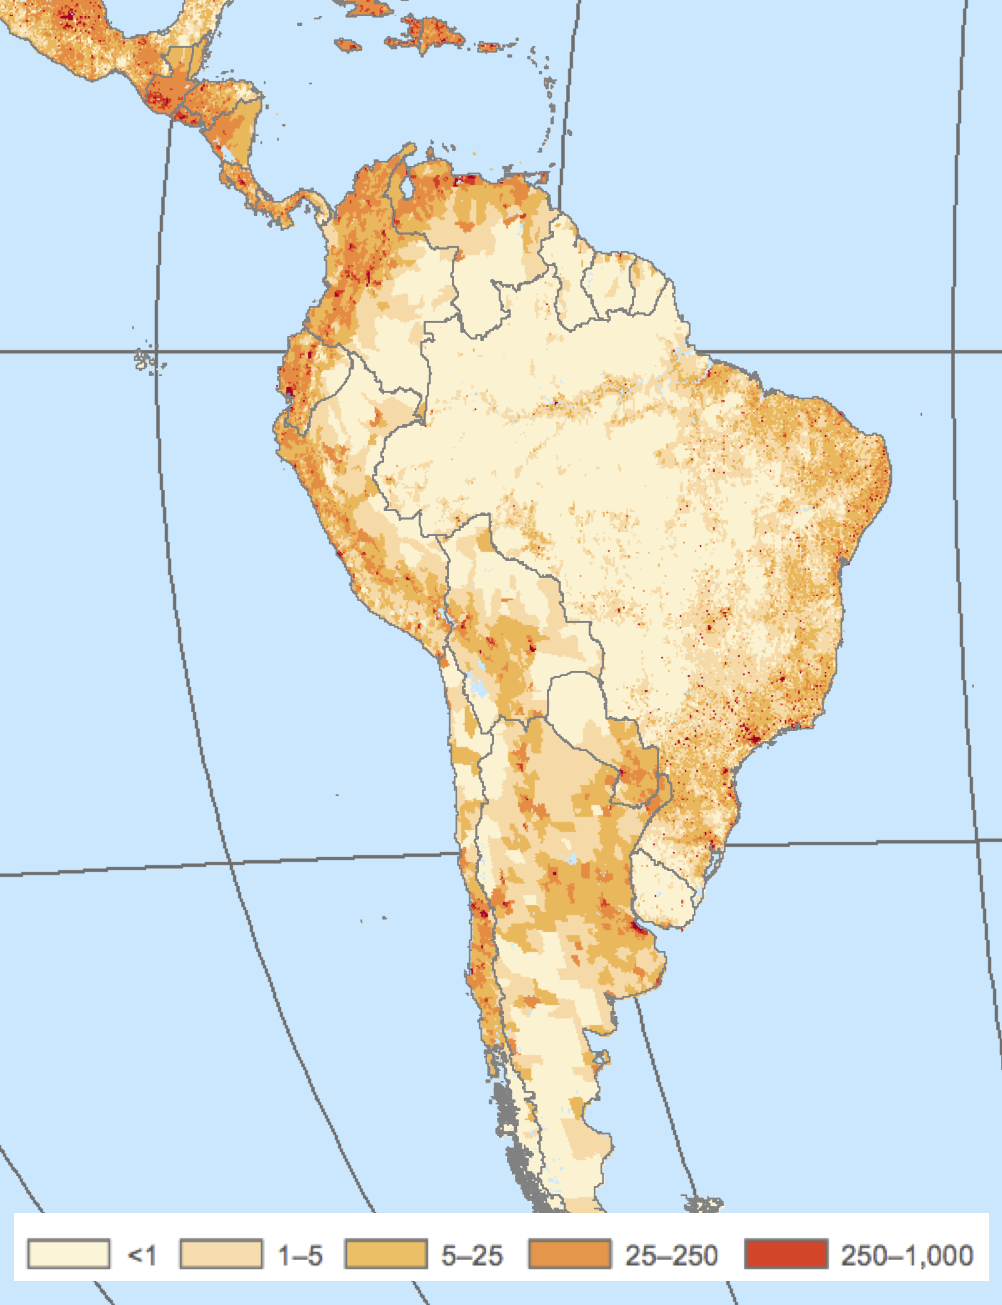
\includegraphics[width=\textwidth,height=0.6\textheight,keepaspectratio=true]{gpw-v4-2015.png}
	\caption{
		Gridded estimate of population density (color; in units of persons per square kilometer) from \citet{GPWv4}.
	}
\end{figure}

\begin{figure}
  \includegraphics[width=\textwidth]{PSI_Var_Explained.pdf}
	\caption{
		Variance explained for each EOF loading of the \SI{850}{\hecto\pascal} streamfunction $\psi$.
    (L): the individual variance explained for each EOF.
		(R): cumulative variance explained.
	}
\end{figure}

\begin{figure}
  \includegraphics[width=\textwidth]{WT_Classifiability.pdf}
	\caption{
		Classifiability index \citep[see Methods and][]{Michelangeli1995} calculated for several chosen values of $K$, representing the number of weather types produced.
		Results are produced with only 50 simulations for each $K$.
	}
\end{figure}

\begin{figure}
  \includegraphics[width=\textwidth]{MJO_Time_Series.pdf}
	\caption{
		Phase plot of the Madden-Julian Oscillation during NDJF 2015-16.
		The $x$-axis shows RMM1 and the $y$-axis shows RMM2 -- gray lines separate MJO phases.
	}
	\label{fig:mjo-ts}
\end{figure}

\clearpage
\bibliographystyle{ametsoc2014}
\bibliography{library}

\end{document}
